\subsection{Encontrando matriz banda p,q}

Como dice el enunciado, cada una de las $2n$ juntas aporta 2 nuevas ecuaciones. El sistema lineal resultante tiene por lo tanto $4n$ ecuaciones con $4n$ incógnitas.
Intuitivamente lo que buscamos es que los números identificadores de las variables que actúan sobre una misma junta sean cercanos entre sí (Eso implica una buena numeración sobre los links de la estructura,
que respresentarán las variables).
Al mismo tiempo queremos que las juntas en donde interviene un determinado link no queden lejos entre sí (Eso implica una buena numeración sobre las juntas de la estructura, que respresentarán las filas).
En primer lugar, para encontrar la matriz banda $B_{p,q}$ dibujamos un puente Pratt Truss de 8 secciones y miramos fijamente la estructura tratando de realizar deducciones al respecto.

\begin{figure}[!h]
	\begin{center}
		  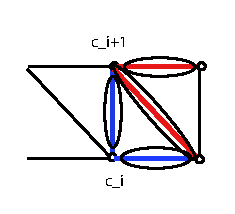
\includegraphics[keepaspectratio]{Imagenes/im_3.pdf}
		  \caption{Cada nuevo par de juntas introduce 4 nuevas fuerzas}
		  \label{fig:contra1}
	\end{center}
\end{figure}
\FloatBarrier

Si miramos a las juntas de a pares verticales: \{c1,c2\}, \{c3,c4\}, \ldots podemos advertir que por cada nuevo par se presentan 4 nuevas fuerzas. A su vez, cada una de las juntas tiene asociada 2 ecuaciones
del sistema (Uno para las fuerzas horizontales y otro para las verticales). Entonces podemos pensar que se introducen 4 nuevas variables cada 4 ecuaciones (1 por ecuación). Por lo tanto, es razonable pensar
que con la numeración correcta podemos llegar a obtener una matriz banda $B_{p,q}$, ya que los coeficientes distintos de cero se concentrarían alrededor de la diagonal. Además, un determinado link solo actúa 
sobre 2 juntas. Indudablemente debemos aprovechar este hecho para establecer el valor $p$ de nuestra matriz. Una numeración razonable consiste en aplicarle (tanto a los links como a las juntas) valores en
forma creciente de izquierda a derecha, y de abajo hacia arriba, tal como está representado en el siguiente diagrama:

\begin{figure}[!h]
	\begin{center}
		  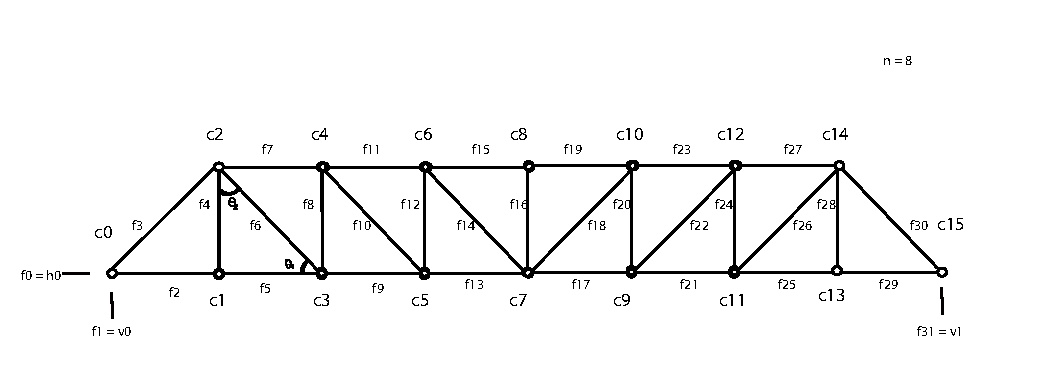
\includegraphics[keepaspectratio]{Imagenes/im_1.pdf}
		  \caption{Numeración para puente de 8 secciones}
		  \label{fig:contra1}
	\end{center}
\end{figure}
\FloatBarrier

Con dicha numeración, renombrando $junta_{i}=c_{i}$ y $link_{j}=f_{j}$, las primeras 6 ecuaciones (correspondientes a las primeras 3 juntas) del sistema lineal obtenido serían:

Ecuación 0: $c_{0} \ = 1*h_{0} + 0*v_{0} + 1*f_{2} + cos(\theta_{1})*f3 + 0*f_{4} + 0*f{5} + 0*f{6} + 0*f_{7} \ldots$

Ecuación 1: $c_{0} v = 0* h_{0} + 1*v_{0} + 0*f_{2} + sen(\theta_{1})*f3 + 0*f_{4} + 0*f{5} + 0*f{6} + 0*f_{7} \ldots$

Ecuación 2: $c_{1} \ = 0* h_{0} + 0*v_{0} - 1*f_{2} + 0*f3 + 0*f_{4} + 1*f{5} + 0*f{6} + 0*f_{7} \ldots$

Ecuación 3: $c_{1} v = 0* h_{0} + 0*v_{0} - 0*f_{2} + 0*f3 + 1*f_{4} + 0*f{5} + 0*f{6} + 0*f_{7} \ldots$

Ecuación 4: $c_{2}  \ = 0* h_{0} + 0*v_{0} - 0*f_{2} - sen(\theta_{2})*f3 + 0*f_{4} + 0*f{5} + sen(\theta_{2})*f{6} + 1*f_{7} \ldots$

Ecuación 5: $c_{2}v  \ = 0* h_{0} + 0*v_{0} - 0*f_{2} - cos(\theta_{2})*f3 - 1*f_{4} + 0*f{5} + cos(\theta_{2})*f{6} + 0*f_{7} \ldots$

~

Los siguientes pares de ecuaciones (luego de analizar las primeras tres juntas, y antes de llegar a las de la mitad de la estructura) comparten una especie de patrón. Notemos en primer lugar que los números
de las ecuaciones correspondientes a analizar la junta $c_{i}$ son $2*i$, correspondiente al plano horizontal y $2*(i+1)$, correspondiente al plano vertical. Además debemos considerar también si la junta es 
inferior o superior.

Si $c_{i}$ es junta inferior, entonces:

Ecuación $(2*i)$ \ \ \ \ \  : $c_{i} = -1*f_{2i-1} - cos(\theta_{1})*f_{2i} + 0*f_{2i+1} + 0*f_{2i+2} + 1*f_{2i+3}$   

Ecuación $(2*i+1)$ : $c_{i} v = sen(\theta_{1})*f_{(2i+1)-1} + 0*f_{2i+1} + 1*f_{(2i+1)+1} + 0*f_{(2i+1)+2} + 0*f_{(2i+1)+3}$

~

Si por el contrario, $c_{i}$ es junta superior entonces:

Ecuación $(2*i)$ \ \ \ \ \  : $c_{i} = -1*f_{2i-1} + 0*f_{2i} + 0*f_{2i+1} + sen(\theta_{2})*f_{2i+2} + 1*f_{2i+3}$   

Ecuación $(2*i+1)$ : $c_{i} v = -1*f_{(2i+1)-1} + 0*f_{2i+1} - cos(\theta_{2})*f_{(2i+1)+1} + 0*f_{(2i+1)+2} + 0*f_{(2i+1)+3}$

~

Las ecuaciones de las juntas del medio: $c_{n-1}$ la inferior y $c_{n}$ la superior deben ser planteadas aparte ya que son distintas al resto:

~

Inferior:

Ecuación $(2(n-1))$ : $c_{n-1} = -1*f_{2(n-1)-1} - cos(\theta_{1})*f_{2(n-1)} + 0*f_{2(n-1)+1} + 0*f_{2(n-1)+2} + 1*f_{2(n-1)+3} + cos(\theta_{1})*f_{2(n-1)+4}$ \\  

Ecuación $(2n-1)$ : $c_{n-1} v = -sen(\theta_{1})*f_{(2n-1)-1} + 0*f_{2n-1} + 1*f_{(2n-1)+1} + 0*f_{(2n-1)+2} + sen(\theta_{1})*f_{(2n-1)+3}$

~

Superior:

Ecuación $(2n)$ : $c_{n} = -1*f_{2n-1} + 0*f_{2n)} + 0*f_{2n+1} + 0*f_{2n+2} + 1*f_{2n+3}$ \\  

Ecuación $(2n+1)$ : $c_{n} v = -1*f_{(2n+1)-1} + 0*f_{2n+1} + 0*f_{(2n+1)+1} + 0*f_{(2n+1)+2} + 0*f_{(2n+1)+3}$

~

Los siguientes pares de ecuaciones vuelven a compartir un patrón (al igual que en la primera parte). Esto sucede para todos los pares restantes, con excepción del último:  

~

Si $c_{i}$ es junta inferior, entonces:

Ecuación $(2*i)$ \ \ \ \ \  : $c_{i} = -1*f_{2i-1} + 0*f_{2i} + 0*f_{2i+1} + 0*f_{2i+2} + 1*f_{2i+3} + cos(\theta_{1})*f_{2i+4}$   

Ecuación $(2*i+1)$ : $c_{i} v = 0*f_{(2i+1)-1} + 0*f_{2i+1} + 1*f_{(2i+1)+1} + 0*f_{(2i+1)+2} + sen(\theta_{1})*f_{(2i+1)+3}$

~

Si por el contrario, $c_{i}$ es junta superior entonces:


~

Finalmente, quedan analizar por separado las últimas 3 juntas: el par \{$c_{2n-3},c_{2n-2}$\} y $c_{2n-1}$: \\

Ecuación $(2(2n-3))$ \ \ : $c_{2n-3} = -1*f_{2(2n-3)-1} + 0*f_{2(2n-3)} + 0*f_{2(2n-3)+1} + 0*f_{2(2n-3)+2} + 1*f_{2(2n-3)+3} $ \\

Ecuación $(2(2n-3)+1 = 4n-5)$ : $c_{2n-3} v = 0*f_{(4n-5)} + 1*f_{(4n-5)+1} + 0*f_{(4n-5)+2} $ \\

Ecuación $(2(2n-2))$ \ \ : $c_{2n-2} = -sen(\theta_{2})*f_{2(2n-2)-2} - 1*f_{2(2n-2)-1} + 0*f_{2(2n-2)} + 0*f_{2(2n-2)+1} + sen(\theta_{2})*f_{2(2n-2)+2} $ \\

Ecuación $(2(2n-2)+1 = 4n-3)$ : $c_{2n-2} v = -cos(\theta_{2})*f_{(4n-3)-3} + 0*f_{(4n-3)-2} - 1*f_{(4n-3)-1} + 0*f_{(4n-3)} + cos(\theta_{2})*f_{(4n-3)+1} $ \\

Ecuación $(2(2n-1))$ \ \ : $c_{2n-1} = -1*f_{2(2n-1)-1} - cos(\theta_{1})*f_{2(2n-1)} + 0*f_{2(2n-1)+1} + 0*f_{2(2n-1)+2}$ \\

Ecuación $(2(2n-1)+1 = 4n-1)$ : $c_{2n-1} v = sen(\theta_{1})*f_{(4n-1)-1} + 1*f_{(4n-1)} + 0*f_{(4n-1)+1} + 0*f_{(4n-1)+2}$ \\


\begin{figure}[!h]
	\begin{center}
		  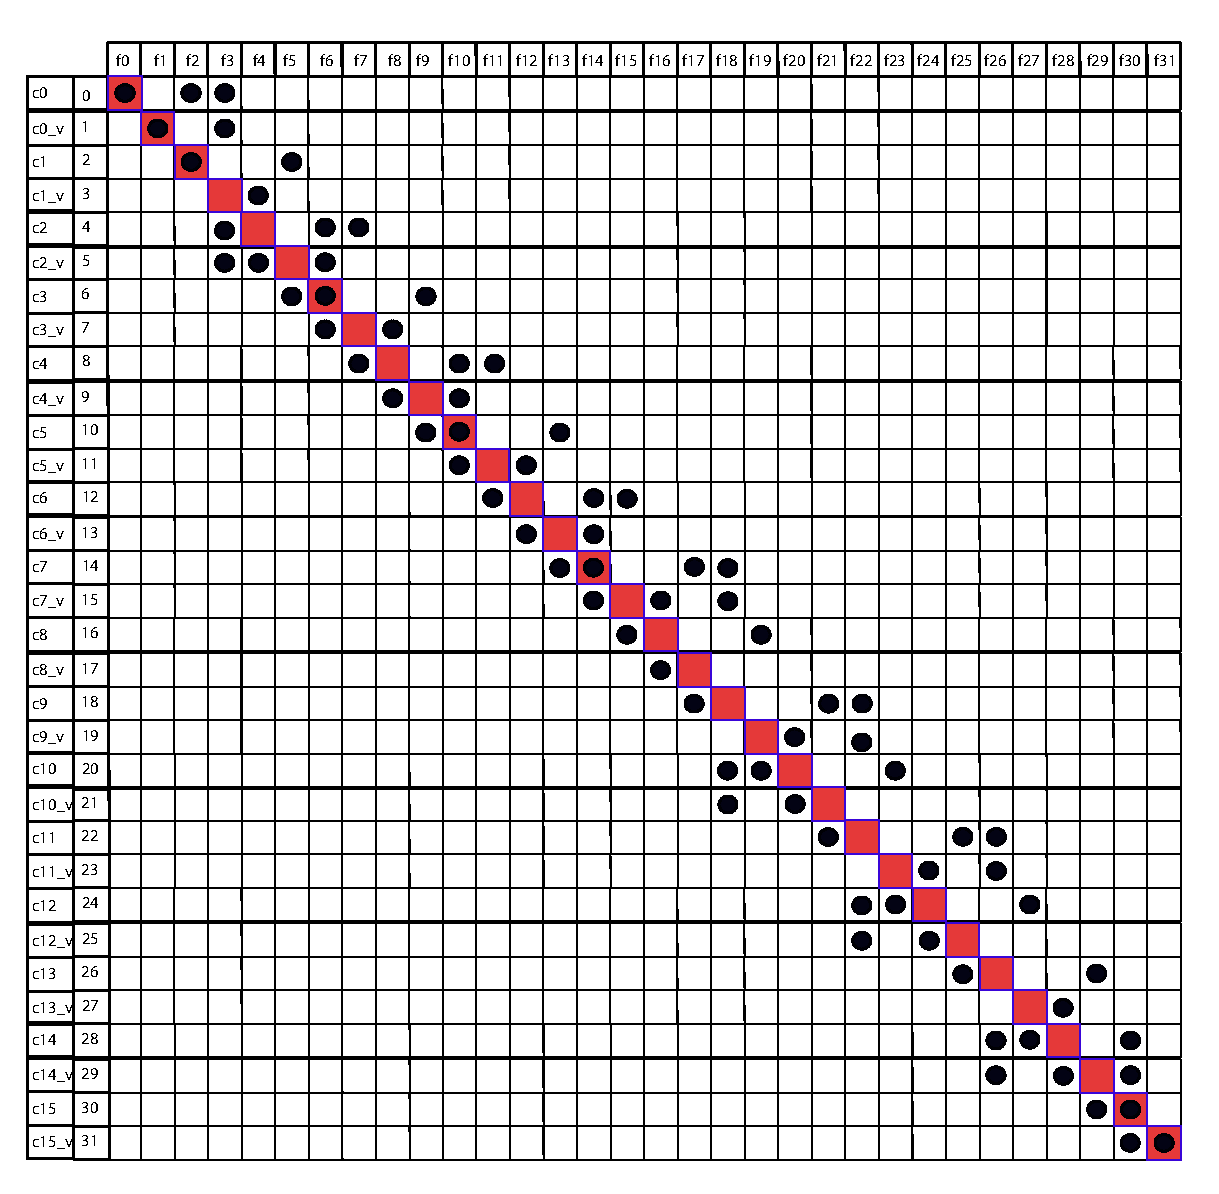
\includegraphics[scale=0.5]{Imagenes/im_2.pdf}
		  \caption{Esquema de matriz a partir del sistema de ecuaciones}
		  \label{fig:contra1}
	\end{center}
\end{figure}
\FloatBarrier

Al mirar el esquema de la matriz podemos llegar a clasificar rápidamente a la matriz como banda 3,4. Tratemos de analizar un poco este hecho:

Sea $b$ nuestra matriz. 
La mitad izquierda de la banda, también conocida como $p$, está relacionada con la mayor distancia entre una fila $i$, y una fila $j$, con $j \geq i$ para 
las cuales el $link_{i}$ interviene en la ecuación de la fila $j$. Por lo tanto, si llamamos $p$ a esta distancia observamos que:

- $b_{j,j-p} \neq 0$. Justamente, $j-p = i$, y habíamos dicho que $link_{i}$ interviene en dicha ecuación.

- Sea $h$ una fila tal que $h \neq j$. Entonces, el índice de la columna más a la izquierda que tiene un coeficiente $\neq 0$ es mayor o igual a (h-p).

\begin{figure}[!h]
	\begin{center}
		  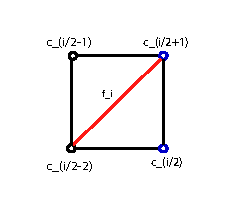
\includegraphics[scale=1.5]{Imagenes/im_4.pdf}
		  \caption{Explicación de la mitad izquierda de la banda: \emph{p}}
		  \label{fig:contra1}
	\end{center}
\end{figure}
\FloatBarrier

En el caso de nuestro puente, las juntas que presentan esta máxima distancia \emph{p} son aquellas como las que muestra la 
figura, pintadas en azul: Par alineado verticalmente perteneciente a la segunda mitad del puente.  

\begin{figure}[!h]
	\begin{center}
		  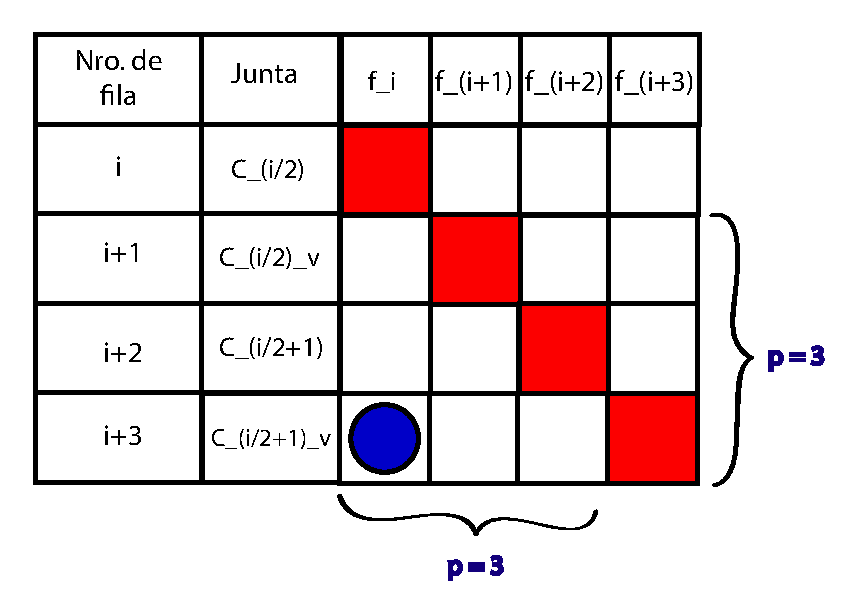
\includegraphics[scale=0.5]{Imagenes/im_5.pdf}
		  \caption{Explicación de la mitad izquierda de la banda: \emph{p}}
		  \label{fig:contra1}
	\end{center}
\end{figure}
\FloatBarrier

Tal como vemos en la figura 5, el coeficiente que acompaña a $f_{i}$ es distinto de cero en la ecuación $i+3$. Esto determina
una banda izquierda $p \leq 3$. Sin embargo, para ningún par de ecuaciones se cumple $p > 3$. Por lo tanto, podemos concluir que $p=3$.

~

La mitad derecha de la banda, conocida como $q$, está relacionada con el link de mayor numeración que interviene en la ecuación
de una junta. Profundizando un poco, al analizar la ecuación $i$, la 
diferencia entre la mayor columna $j$ y la columna $i$ (con $j \geq i$ tal que $b_{i,j} \neq 0$)
determina la mitad derecha de la banda para dicha ecuación. La mayor de estas diferencias para todas las filas determina $q$.

\begin{figure}[!h]
	\begin{center}
		  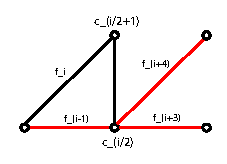
\includegraphics[scale=1.5]{Imagenes/im_6.pdf}
		  \caption{Explicación de la mitad derecha de la banda: \emph{q}}
		  \label{fig:contra1}
	\end{center}
\end{figure}
\FloatBarrier

Tal como muestra el esquema, esta máxima diferencia se produce en las ecuaciones horizontales pertenecientes a las juntas
inferiores de la segunda mitad del puente. 

\begin{figure}[!h]
	\begin{center}
		  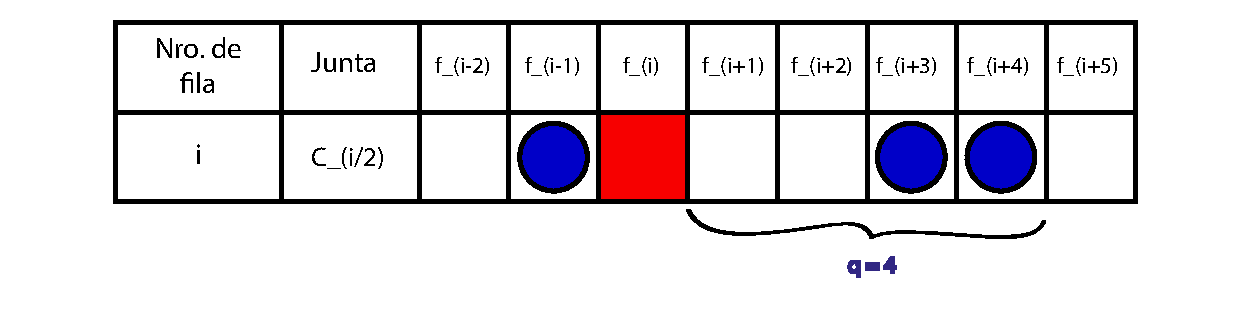
\includegraphics[scale=0.5]{Imagenes/im_7.pdf}
		  \caption{Explicación de la mitad derecha de la banda: \emph{q}}
		  \label{fig:contra1}
	\end{center}
\end{figure}
\FloatBarrier

Al analizar la fila $i$, perteneciente a la ecuación horizontal de la junta $\frac{i}{2}$, el link de mayor numeración que
interviene en la ecuación es $i+4 \Rightarrow \ q \geq 4$. Sin embargo, para ninguna ecuación esta diferencia es mayor que 
4, por lo que podemos concluir que $q=4$.


Hemos probado entonces que nuestra matriz es banda 3,4. Sin embargo durante la aplicación 
de eliminación Gaussiana con pivoteo parcial eventualmente será necesario realizar intercambio de filas. 
Demostremos que luego de aplicar este método sobre una matriz banda $b_{p,q}$, la matriz resultante es banda $b_{p,(p+q)}$


\subsection{Demostración por inducción sobre el i-ésimo paso de la eliminación Gaussiana}

~

Sea $b_{p,q} \in R^{nxn}$, y sea $b^{i}$ la matriz resultante luego de aplicar el i-ésimo paso de eliminación Gaussiana con
pivoteo parcial. Probemos que al finalizar el método, la matriz $b^{n-1}$ obtenida es banda p, q+p.

~

\subsubsection{Caso base}

~

En el primer paso del método pueden suceder 2 cosas:

1) No se produce pivoteo sobre la primera fila $\Rightarrow$ demostración es trivial.

2) Se produce el intercambio entre la fila 1 y una fila $j$ con $1<j \leq (p+1)$. 

~

\underline{Bandas en la fila j al intercambiar fila 1 con fila j:}

La banda izquierda está determinada por la diferencia entre $j$ y la columna de menor índice que contenga un elemento distinto
de cero: llamemos a este índice $i$. Notemos que en el peor caso $i=1$ $\Rightarrow$ Banda izquierda = $j-i \leq (p+1) - i \leq
(p+1) - 1 = p$. (El máximo ancho de banda ''izquierda'' se produce al intercambiar la primera fila con la $p+1$.)

La banda derecha está determinada por la diferencia entre la columna de mayor índice $k$
que contenga un elemento distinto de cero y $j$ . Notemos que en el peor caso $j=2$ y $k =1+q$ $\Rightarrow$ Banda derecha =
$k-j \leq (1+q) -2 = (q-1)$. (El máximo ancho de banda ''derecha'' se produce al intercambiar la primera fila
con la segunda)

Por lo tanto la fila $j$ (en cualquiera de los casos) mantiene la propiedad de ser banda p,(p+q).

~

\underline{Bandas en la fila 1 al intercambiar fila 1 con fila j:}

Como estamos analizando la primera fila, es inmediato ver que la banda izquierda continúa siendo $p$, ya que no hay elementos
a la izquierda de la columna 1.

La banda derecha está determinada por la diferencia entre la columna de mayor índice $k$ que contenga un elemento distinto
de cero y la columna 1. Notemos que en el peor caso $j=1+p$ y $k=j+q$ $\Rightarrow k-1 = 1+p+q-1 = p+q$. (El máximo ancho de 
banda ''derecha'' se produce al intercambiar la primera fila con la $p+1$.)

Por lo tanto, la primera fila mantiene la propiedad de ser banda p,(p+q).

~

Sea $k$ una fila tal que $1 \leq k \leq (p+1)$. Luego de realizar el primer paso de Gauss y generar los ceros en la 
primera columna tenemos que:

- Banda izquierda de k $\leq (k-1) \leq (p+1)-1 = p$

- Banda derecha de k $ \leq (1+p+q)-k \leq p+q $

Como el resto de las filas no han sido modificadas, podemos afirmar que $b^{1}$ es banda p,(p+q). 
Demostrado caso base $\square$

~

\subsubsection{Paso inductivo: $P(i-1) \Rightarrow P(i)$}

~

Sea $j$ tal que $0 \leq j \leq (p-1)$. Analicemos brevemente qué sucede con cada una de las filas $i+j$.
En la matriz inicial $b^{0}$ sabíamos que el elemento más a la derecha para cada una de ellas estaba a lo sumo en la columna:
$i+j+q$. Sin embargo esta situación pudo haber cambiado luego de realizar el paso (i-1)-ésimo. En esta instancia, el
elemento más a la derecha podría estar a lo sumo en la columna: $i+p+q-1$. Notemos que $i+j+q \leq i+p+q-1 , \ \forall 
\ 0 \leq j \leq (p-1)$.

\begin{figure}[!h]
	\begin{center}
		  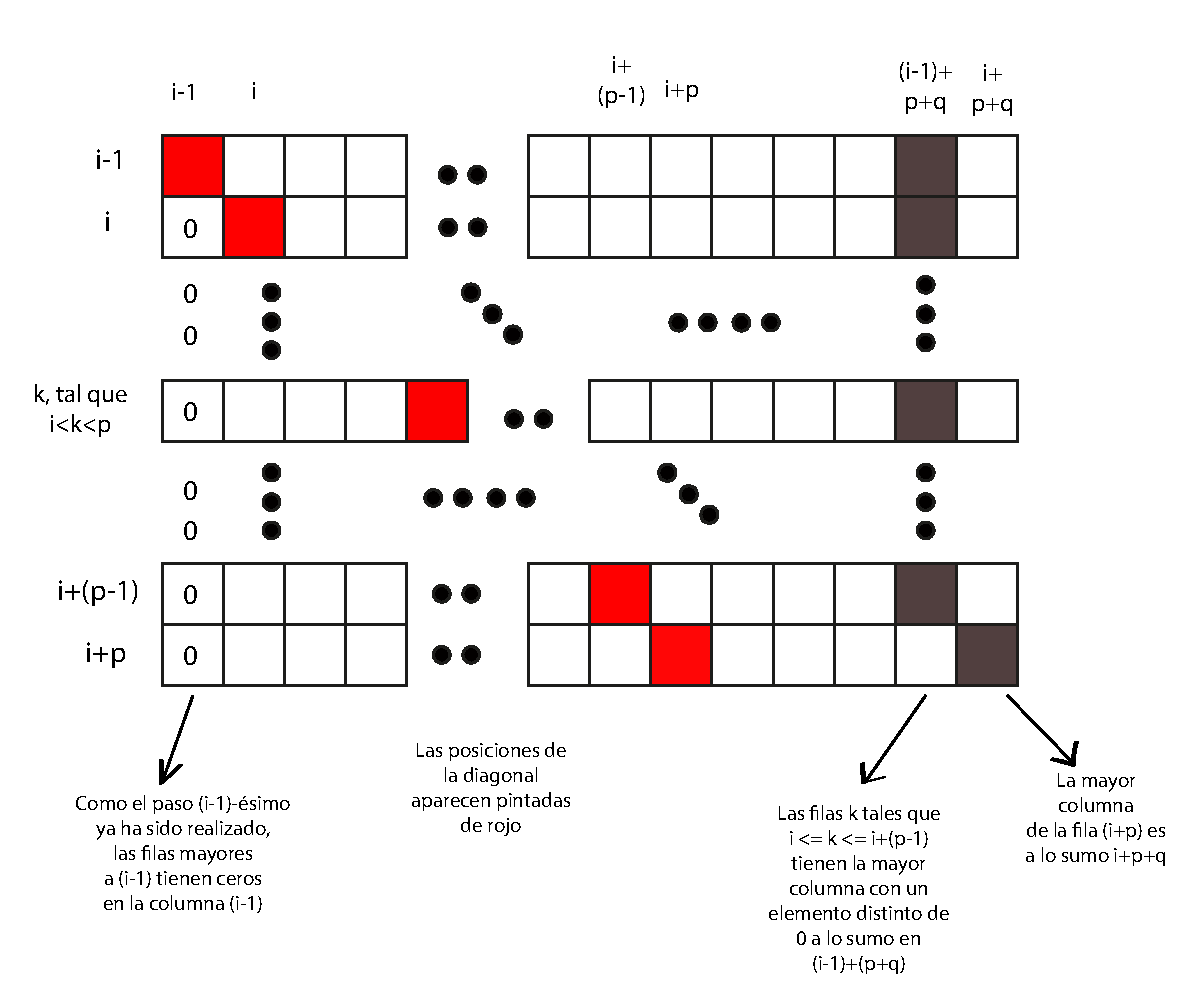
\includegraphics[scale=0.5]{Imagenes/im_8.pdf}
		  \caption{Estado de la matriz luego de realizar el (i-1)-ésimo paso. Se muestran únicamente
		  las filas y columnas que intervienen en el i-ésimo paso}
		  \label{fig:contra1}
	\end{center}
\end{figure}
\FloatBarrier

Para la fila $(i+p)$ la columna de mayor índice es a lo sumo $(i+p+q)$. Es suficiente probar que la matriz se mantiene como 
banda (p,p+q) luego de intercambiar las filas $i$ e $i+p$ ya que constituye el peor caso que podría ensanchar las bandas.

\begin{figure}[!h]
	\begin{center}
		  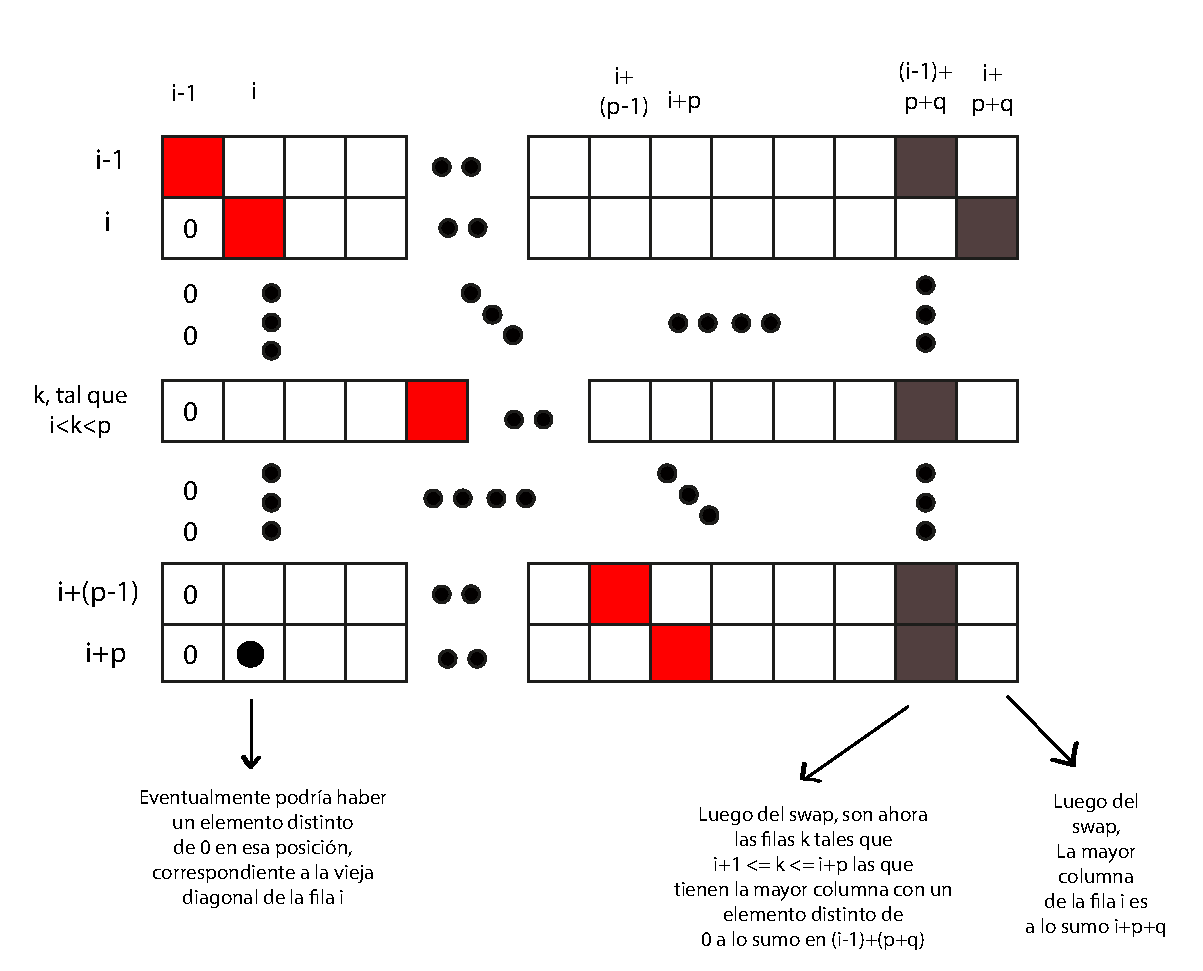
\includegraphics[scale=0.5]{Imagenes/im_9.pdf}
		  \caption{$b^{(i-1)}$ al swapear las filas i e (i+p), ya que constituye el peor caso que podría ensanchar
		  las bandas.}
		  \label{fig:contra1}
	\end{center}
\end{figure}

~

\underline{Bandas en la fila $i$ al intercambiar fila $i$ con fila $i+p$}

$Banda \ izquierda \leq i - (i+p-p) = 0$ (Columna de la diagonal menos columna del elemento más a la izquierda)

$Banda \ derecha \leq (i+p+q) - i = p+q$ (Columna del elemento más a la derecha menos columna diagonal)

La fila $i$ mantiene la propiedad de ser banda p,(p+q).

~

\underline{Bandas en la fila $i+p$ al intercambiar fila $i$ con fila $i+p$}

Como ya se han puesto ceros en las columnas a la izquierda de la i-ésima, tenemos que:

$Banda \ izquierda \leq (i+p) - (p) = 0$ (Columna de la diagonal menos columna del elemento más a la izquierda)

$Banda \ derecha \leq (i+p+q-1) - (i+p) \leq p+q$ (Columna del elemento más a la derecha menos columna diagonal)

La fila $(i+p)$ mantiene la propiedad de ser banda p,(p+q).

~

\begin{figure}[!h]
	\begin{center}
		  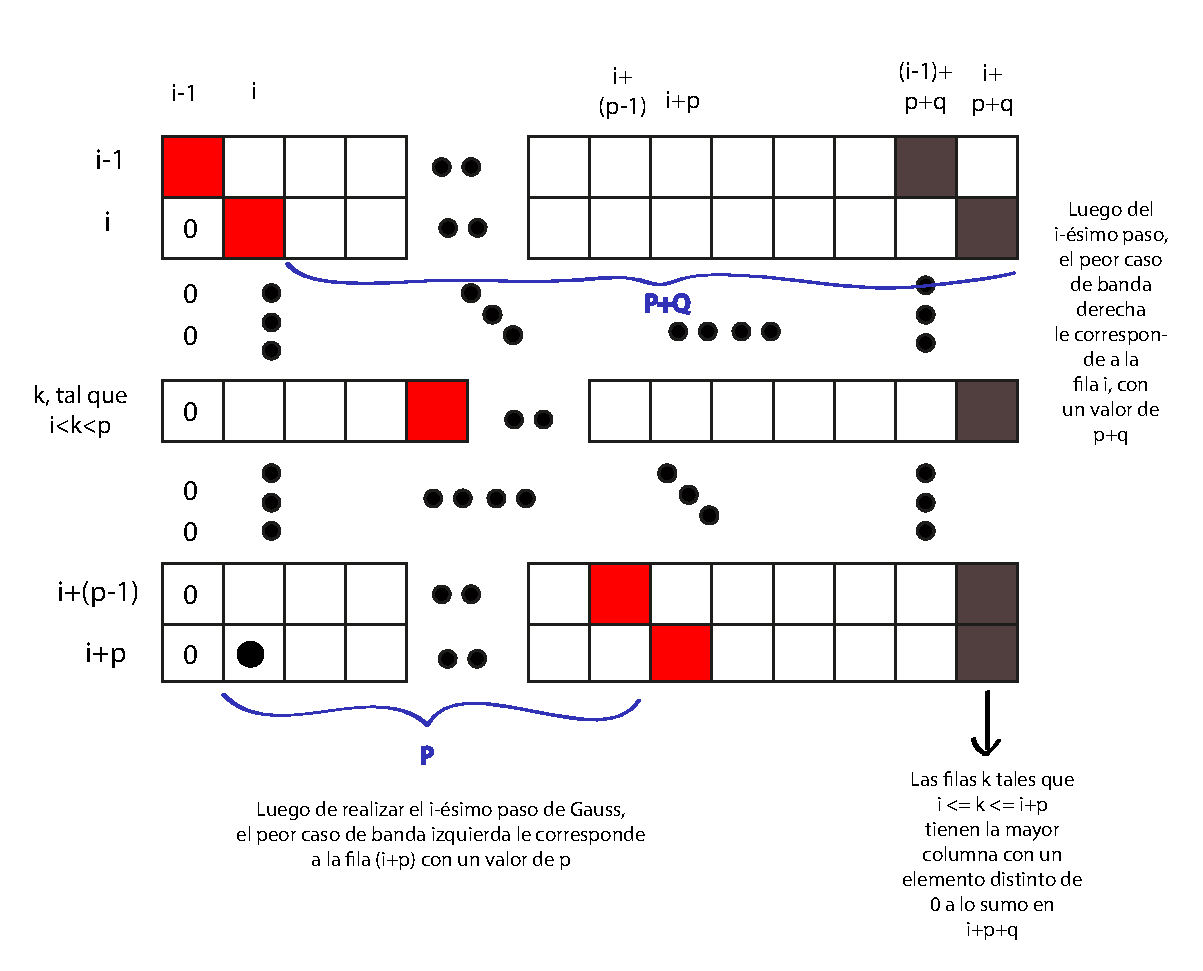
\includegraphics[scale=0.5]{Imagenes/im_10.pdf}
		  \caption{$b^{(i)}$ al realizar el paso habiendo intercambiado las filas i e (i+p)}
		  \label{fig:contra1}
	\end{center}
\end{figure}

Sea $k$ una fila tal que $i \leq k \leq (i+p)$. Luego de realizar el i-ésimo paso de Gauss y generar los ceros en la 
i-ésima columna tenemos que:

- Banda izquierda de k $\leq (k-i) \leq (i+p)-i = p$

- Banda derecha de k $ \leq (i+p+q)-k \leq (i+p+q)-i = p+q $

Como el resto de las filas no han sido modificadas, podemos afirmar que $b^{i}$ es banda p,(p+q). 
Demostrado paso inductivo $\square$

\subsection{Experimentación}

Luego de implementar el algoritmo de eliminación Gaussiana con pivoteo parcial adaptado a nuestra representación de la matriz banda,
realizamos experimentos para ver qué sucedía con las fuerzas ejercidas sobre cada link en base a lo pedido por el enunciado:

a) Variando el \emph{span}, con la altura y el peso de las cargas fijo, para distintos valores de \emph{n}.

b) Variando el peso de las cargas, con el \emph{span} y la altura fijos, para distintos valores de \emph{n}.

Realizamos ambas etapas de la experimentación variando \emph{n} (que representa la cantidad de secciones de nuestro puente).
Las pruebas fueron realizadas para valores de $n= 4,6,8,10,12$ (valores relativamente peque\~nos, con granularidad de 2), pero 
también con $n=16,32,64,128$ (granularidad mayor).

La parte b) de la experimentación se divide a su vez en otras 3 partes, ya que hay varias maneras de variar el peso de las cargas: 

1) Modificando solamente el peso de una de las ellas, dejando a las restantes con igual peso.

2) Variando uniformemente el peso de todas las cargas.

3) Variando únicamente el valor de la carga de la junta del medio de la estructura.

Decidimos separar la sección b) en estas 3 partes para poder corroborar algunas de nuestras hipótesis o simplemente observar 
los resultados:

1) Hipótesis: Al aumentar el peso de una carga aplicada sobre una $junta_{i}$, existe algún/algunos links en la estructura que se ven
particularmente afectados.

2) Observación: Determinar cómo aumentan las fuerzas ejercidas sobre los links a medida que aumenta
el peso de las cargas aguantado por la estructura.

3) Observación: Comparar el crecimiento de las fuerzas ejercidas sobre los links cuando aumenta el peso sobre todas las juntas respecto al
crecimiento cuando aumenta el peso únicamente sobre la junta del medio. Además:
Hipótesis: Variar únicamente el peso de la carga sobre la junta del medio debería mantener la simetría de las fuerzas aplicadas sobre
los links de toda la estructura.

Finalmente, la hipótesis inicial planteada para la parte a) consistió en que, a medida que se incrementa el \emph{span} las fuerzas
ejercidas aumentan también.

(Aclaración: cuando decimos ''las fuerzas aumentan'' nos referimos al módulo de las mismas)



\subsection{Heurística}

Finalmente, luego de realizar la experimentación procedimos a implementar el método heurístico. El mismo se basa fuertemente
en los resultados experimentales obtenidos.

La idea es la siguiente:

- Cuando las cargas están distribuídas de manera uniforme se intenta ubicar un pilar en el medio para intentar reducir el
\emph{span} de ambas sub-estructuras (ya que la magnitud de las fuerzas aumenta con el \emph{span}).

- Por el contrario, cuando hay una carga mayor en módulo que las demás se intenta ubicar un pilar en dicha posición,
ya que el link más afectado probablemente esté en un lugar cercano a la junta sobre la cual se aplica la carga.

\subsection{Aclaraciones}

Incluímos al final del informe los pseudocódigos de las funciones relacionadas con la matriz banda y de la heurística.
